\section{Robust Minimal Recursion Semantics}
\label{sec:rmrs}

We will now make the basic ideas from Section \ref{sec:motivation}
more precise.  We will first define the syntax of the \rmrs\ language;
this is a notational variant of earlier definitions in the
literature.  We will then define a model theory for our version of
\rmrs, and conclude this section by carrying over the notion of
\emph{solved forms} from {\sc clls} \cite{egg:etal:2001}.



\subsection{RMRS Syntax}

We define the syntax of \rmrs\ in the style of {\sc clls}
\cite{egg:etal:2001}.  We assume an infinite set of {\em node
  variables} $\nvar=\{X,Y,X_1,\ldots\}$, used as labels,
anchors, and holes; the distinction between these uses will come from
their position in the formula.  Furthermore, we assume an infinite set
of \emph{base variables} $\ovar$, consisting of individual variables
$\{x,x_1,y,\ldots\}$ and event variables $\{e_1,\ldots\}$.  Finally,
we assume a vocabulary of \emph{predicate symbols}
$\pred=\{P,Q,P_1,\ldots\}$.

We can now define formulas of \rmrs\ as follows.

\begin{definition}\label{defn:rmrs-syntax}
  An \emph{\rmrs} is a finite set $\varphi$ of atoms of one of the
  following forms; $S \subseteq \N$ is a set of numbers that is either
  finite or $\N$ itself.

$\begin{array}{rrll}
A &::= &\ep{X}{Y}{P} \\ %& \mbox{labelled elementary predication} \\
&| &\ARG_S(X,v) \\ % & \mbox{ARG relation for base variables} \\
&| &\ARG_S(X,Y) \\ % & \mbox{ARG relation for node variables} \\
&| &X \qeq Y \\ % & \mbox{QEQ} \\
&| &v_1 = v_2 \;|\; v_1 \neq v_2 \\ % & \mbox{base variable
                                % (in)equality} \\
&| &X = Y \;|\; X \neq Y \\ % & \mbox{node variable (in)equality} \\
&| &P \spec Q % & \mbox{SPEC relation between predicate symbols}
\end{array}
$

A node variable $X$ is called a \emph{label} iff $\varphi$ contains an
atom of the form 
$\ep{X}{Y}{P}$ or $Y \qeq X$; $X$ is called an
\emph{anchor} in the \rmrs\
$\varphi$ iff $\varphi$ contains an atom of the form
$\ep{Y}{X}{P}$ or $\ARG_S(X,i)$; and $X$ is
called a \emph{hole} iff 
$\varphi$ contains an atom of the form $\ARG_S(Y,X)$ or $X \qeq Y$.

An \rmrs\ $\varphi$ is called \emph{normal} iff it satisfies the
following conditions:
\begin{enumerate}
\item Every node variable in $\varphi$ is either a label, an anchor,
  or a hole, but not two of these.
\item If $\ep{X}{Y}{P}, \ep{Z}{Y}{Q}\in \varphi$, then $X=Z$ and $P=Q$
  (i.e., each predication has a unique anchor).
\end{enumerate}
\end{definition}

\rmrs\ as presented here combines similarities to earlier
presentations of \rmrs\ (e.g., \cite{copestake:2003}) and to dominance
constraints \cite{egg:etal:2001}.  We use $\ARG_{\{i\}}$ (with a singleton
set $S$) instead of $\ARG_i$, and $\ARG_\N$ instead of $\ARG_n$.
The elementary predication $\ep{l}{a}{P(v)}$ (see
(\ref{ex:cat-pos})--(\ref{ex:cat-erg})) is a
notational variant of $\{\ep{l}{a}{P}, \ARG_{\{0\}}(a,v)\}$.  In other
words, the syntax defined here differs in some details, but is more
general. The primary differences to dominance constraints are the
distinction of labels and anchors that will separate the labelling and
the parent-child relations, and the use of $\qeq$ instead of
dominance.  Redefining \rmrs\ in the style of dominance constraints
simplifies the formal work below.

\subsection{Model Theory}

The model theory formalises the relationship between an {\sc rmrs} and
the fully specific, alternative logical forms that it describes,
expressed in the base language.  We represent such a logical form as a
tree $\tau$, such as the ones in Fig.~\ref{fig:1}.  So models of the
\rmrs\ are such trees, and we can define satisfaction and entailment
over these models in the usual way.  Satisfaction corresponds to an
\rmrs\ being a partial description of the (unique) fully specific
semantic representation that the model corresponds to, whereas
entailment corresponds to the relation between a more and a less
specific \rmrs.

In this paper, we assume for simplicity that the base language is
predicate logic (e.g., see (\ref{ex:fat-cat-1}) and
(\ref{ex:fat-cat-2})); in this case, $\tau$ is simply the structure
tree of 
the predicate logic formula.  We assume that $\Sigma$ is a ranked
signature consisting of predicate logic's symbols: a unary constructor
$\neg$ and binary constructors $\wedge$, $\rightarrow$, etc.; the
binary constructors $\forall x$ and $\exists x$ for all base-language
variables $x$; all the constants and base-language variables are
nullary constructors; and, for each predicate symbol $P$ of arity $n$,
a constructor $P$ of arity $n$.  Other base languages may require a
different signature $\Sigma$ and/or a different mapping between
formulas and trees.  We only assume for convenience that the signature
contains a binary constructor $\wedge$ to represent conjunction.  We
write $\Sigma_i$ for the set of all constructors in $\Sigma$ that have
arity $i$.  We will follow the typographical convention that
non-logical symbols in $\Sigma$ are written in
$\mathsf{sans{-}serif}$, as opposed to the \rmrs\ predicate symbols
like ``$\sempred{\_cat\_n}$'' and ``$\sempred{\_cat\_n\_1}$''.

The models of {\sc rmrs} are then defined to be finite constructor
trees:
\begin{definition}\label{defn:models}
  A {\em finite constructor tree} $\tau$ is a function $\tau:D
  \rightarrow \Sigma$ such that $D$ is a \emph{tree domain} (i.e., a
  subset of $\N^*$ which is closed under prefix and left sibling) and
  the number of children of each node $u \in D$ is equal to the arity
  of $\tau(u)$.  
\end{definition}


We write $D(\tau)$ for the tree domain of a constructor tree $\tau$,
and further define the following relations between nodes in a finite
constructor tree:

\begin{definition}\label{defn:dominance}
$u \qeqdom v$ iff $v = u \cdot 2^k$ for some $k \geq 0$ and all
  symbols $\tau(u), \tau(u \cdot 2), \ldots, \tau(u \cdot 2^{k-1})$
  are quantifiers.  (This is the ``qeq'' relation familiar from
  \newcite{copestake:etal:2005}).

  $u \wedgedom v$ iff $u \leq v$ (i.e.\ it is a prefix), and all
  symbols on the path from $u$ to $v$ (not including $v$) are
  $\wedge$.
\end{definition}

The {\em satisfaction} relation between an \rmrs\ $\varphi$ and a
finite constructor tree $\tau$ is defined in terms of several
assignment functions.  First, we assume a node variable assignment
function $\alpha: \nvar \rightarrow D(\tau)$ that maps the node
variables in an \rmrs\ to the nodes of $\tau$.  Second, we assume a
base language assignment function $g:\ovar \rightarrow \Sigma_0$ that
maps the base variables in the \rmrs\ to nullary constructors
representing variables in the base language.  This function enables us
to map two variables that seem different in the \rmrs\ to the same
base-language variable, introducing e.g.\ semantic dependencies that a
POS tagger didn't catch.  For instance, $g$ might map $x_4$ and $x_5$
in (\ref{ex:cat-pos}) to $y$ to specify a variable binding.  Finally,
we assume a relation $\sigma \subseteq \pred \times \Sigma_{\geq 1}$
that maps each \rmrs\ predicate symbol to a set of constructors from
$\Sigma$.  This relation allows us to underspecify lexical
ambiguities; for instance, $\sigma(\sempred{\_cat\_n})$ might contain
the symbol $\sem{\_cat\_n\_1}$ along with symbols for other word
senses.

\begin{definition}\label{defn:satisfaction}
Satisfaction of atoms is defined as follows:
$$
\begin{array}{l}
  \tau, \alpha, g, \sigma \models  \ep{X}{Y}{P}
\mbox{ iff}\\
\qquad \tau(\alpha(Y)) \in \sigma(P) \mbox{ and } \alpha(X) \wedgedom
  \alpha(Y) \\
  \tau, \alpha, g, \sigma \models \ARG_S(X,a)
\mbox{ iff exists  $i \in S$ s.t.}\\
\qquad  \alpha(X) \cdot i \in D(\tau) \mbox{ and }
  \tau(\alpha(X) \cdot 
  i) = g(a) \\
  \tau, \alpha, g, \sigma \models \ARG_S(X,Y)
\mbox{ iff  exists $i \in S$ s.t.}\\
\qquad \alpha(X) \cdot i \in D(\tau), \alpha(X) \cdot
  i = \alpha(Y)\\
  \tau, \alpha, g, \sigma \models X \qeq Y
\mbox{ iff } \alpha(X) \qeqdom \alpha(Y) \\
  \tau, \alpha, g, \sigma \models X ={/}\neq Y
\mbox{ iff } \\
\qquad \alpha(X) ={/}\neq \alpha(Y) \\
  \tau, \alpha, g, \sigma \models v_1 ={/}\neq v_2
\mbox{ iff}\\
\qquad g(v_1) ={/}\neq g(v_2) \\
  \tau, \alpha, g, \sigma \models P \spec Q
\mbox{ iff $\sigma(P) \subseteq \sigma(Q)$}
\end{array}
$$
A 4-tuple $\tau,\alpha,g,\sigma$ satisfies an \rmrs\ $\varphi$
(written $\tau,\alpha,g,\sigma \models \varphi$) iff it satisfies all
of its elements.
\end{definition}

Notice that one \rmrs\ may be satisfied by multiple trees; we can take
the \rmrs\ to be a partial description of each of these trees.  In
particular, \rmrs s may represent semantic scope ambiguities, and/or missing
information about semantic dependencies, 
lexical subcategorisation and lexical senses.  For $j=\{1,2\}$,
suppose that $\tau_j,\alpha_j,g_j,\sigma\models \varphi$ and let
$\nvar$ and $\ovar$ be the node and base variables from which
$\varphi$ is built.  Then 
$\varphi$ exhibits a semantic scope ambiguity if there are variables
$Y,Y'\in \nvar$ such that $\alpha_1(Y) \qeqdom \alpha_1(Y')$ and
$\alpha_2(Y')\qeqdom \alpha_2(Y)$.  It exhibits missing information
about semantic dependencies if there are base-language variables
$v,v'\in \ovar$ such that $g_1(v)=g_1(v')$ and $g_2(v)\neq g_2(v')$. 
It exhibits missing lexical subcategorisation information if there is
a $ Y \in \nvar$ such that $\tau_1(\alpha_1(Y))$ is a
constructor of a different type from $\tau_2(\alpha_2(Y))$  (i.e., the
constructors are of a different arity and/or their arguments are).
And it exhibits missing lexical sense information
if $\tau_1(\alpha_1(Y))$ and $\tau_2(\alpha_2(Y))$ are different
base-language constructors, but of the same type.

Let's look at the \rmrs\ in (\ref{ex:cat-pos}) by way of example.
This \rmrs\ is satisfied by the trees in Fig.~\ref{fig:1} (among
others) together with some particular $\alpha$, $g$, and $\sigma$.
For instance, consider the left-hand side tree in Fig.~\ref{fig:1}.
The \rmrs\ (\ref{ex:cat-pos}) satisfies this tree with an assignment
function $\alpha$ that maps the variables $l_1$ and $a_1$ to the
root node, $l_{41}$ and $l_{42}$ to its second child (labeled with
``$\wedge$''), $a_{41}$ to the first child of \emph{that} node (i.e.\
the node 21, labelled with ``fat'') and $a_{42}$ to the node 22, and
so forth.  $g$ will map $x_1$ and $x_3$ to $x$, and $x_6$ and $x_7$ to
$y$, and so on.  
And $\sigma$ will map each \rmrs\ predicate symbol (which represents a
word) to the set of its word senses, e.g.\ \_cat\_n to a set
containing $\sem{\_cat\_n\_1}$ and possibly others.  It is then easy to verify
that every single atom in the \rmrs\ is satisfied---most
interestingly, the {\sc ep}s $\ep{l_{41}}{a_{41}}{\_fat\_a(e')}$ and
$\ep{l_{42}}{a_{42}}{\_cat\_n(x_3)}$ are satisfied because
$\alpha(l_{41}) \wedgedom \alpha(a_{41})$ and $\alpha(l_{42})
\wedgedom \alpha(a_{42})$.

Truth, validity and entailment can now be defined in terms of
satisfiability in the usual way:
\begin{definition}\label{defn:entailment}
\begin{description}
\item   [truth:] $\tau\models \varphi$ iff $\exists \alpha,g,\sigma$  such
  that $\tau,\alpha,g,\sigma\models \varphi$
\item   [validity:] $\models \varphi$ iff $\forall \tau$, $\tau\models \varphi$.
\item   [entailment:] $\varphi\models \varphi'$ iff $\forall \tau$, if
  $\tau\models \varphi$ then $\tau\models \varphi'$.
\end{description}
\end{definition}
% NOTE: This definition of entailment isn't right, because it allows
% the assignment $\sigma$ from predicates to constructors to vary
% when testing the satisfiability of $\varphi$ vs. $\varphi'$ with
% respect to $\tau$.  I think that to get the notion of entailment we
% want, $\sigma$ should actually be part of the {\sc rmrs} *model*.
% In other words, an {\sc rmrs} model $M$ is a tuple $\langle \tau,
% \sigma\rangle$, where $\tau$ is a finte constructor tree and
% $\sigma$ is a mapping from $\Pred$ to the power set of $\Sigma$.
% Then truth and entailment are defined correctly.  I believe our
% proofs of things like Theorem~\ref{thm:big-one} actually assumes
% that $\sigma$ is constant when interpreting $\varphi$ vs.\
% $\varphi'$, no?



\subsection{Solved Forms}

One feature which the above definition of \rmrs\ shares with dominance
constraints is that any satisfiable \rmrs\ has an infinite number of
models which only differ in the areas that the \rmrs\ didn't ``talk
about''.  An example is shown in Fig.~\ref{fig:fat-black-cat}.  This
tree, which represents the meaning of ``every fat black cat chased
some dog'', is still a model
of (\ref{ex:cat-pos})---all the {\sc ep}s are satisfied.  However, there is
more ``semantic material'' (the ``black'' subformula).  The \rmrs\
didn't specify that this material should be there; but it also didn't
specify that it can't be there, and indeed there is no way in which
the \rmrs\ can enforce that no extra material can be added (e.g.,
consider predicate symbols that are introduced by construction rules
in a deep grammar, which by design are absent from the semantic output
of a {\sc pos} tagger).


\begin{figure}
  \centering
  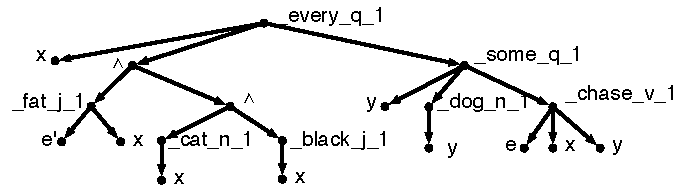
\includegraphics[width=6cm]{pic-more-stuff}
  \caption{Another tree which satisfies (\ref{ex:cat-pos}).}
  \label{fig:fat-black-cat}
\end{figure}


In the context of robust semantic processing, this is a desirable
feature of \rmrs, because it means that when we enrich an \rmrs\
obtained from a shallow processor with more semantic information, we
don't change the set of models; we only \emph{restrict} the set of
models further and further towards the semantic representation we are
trying to reconstruct.  However, the fact that all satisfiable \rmrs s
have an infinite number of models is a problem for algorithms that try
to decide satisfiability or compute the fully specific semantic
representations---how can this be done in finite time?

In this paper, we follow the dominance constraint strategy for
resolving this dilemma; we
define a fragment of \rmrs s called \emph{solved forms}.  All \rmrs
s in solved form are guaranteed to be satisfiable, and thus each
solved form represents an infinite class of models.  However, we will
set it up in such a way that each satisfiable \rmrs\ has only a finite
number of solved forms which partition the space of possible models
into classes with only ``irrelevant'' differences as above.  A solver
can then enumerate the solved forms rather than all models.

Intuitively, we expect that an \rmrs\ in solved form is fully
specified with respect to the predicate-argument
structure, all variable equalities and inequalities have been
resolved, and only lexical sense ambiguities and (resolvable)
scope ambiguities remain.  This is made
precise below.


\begin{definition}\label{defn:solved-forms}
  An RMRS $\varphi$ is \emph{in solved form} iff:
  \begin{enumerate}
  \item every variable in $\varphi$ is either a hole, a label or an
    anchor (but not two of these);
  \item $\varphi$ doesn't contain equality, inequality, and SPEC
    ($\sqsubseteq$) atoms;
  \item if $\ARG_S(Y,i)$ is in $\varphi$, then $|S| = 1$;
  \item for any label $Y$ and index set $S$, there
    are no two atoms $\ARG_S(Y,i)$ and $\ARG_S(Y,i')$ in $\varphi$;
  \item if $Y$ is an anchor in some {\sc ep} $\ep{X}{Y}{P}$ and $k$ is the
    maximum number such that $\ARG_{\{k\}}(X,i)$ is in $\varphi$ for
    any $i$, then there is a constructor $p \in \sigma(P)$ whose arity
    is at least $k$;
  \item no label occurs on the right-hand side of two
    different $\qeqdom$ atoms.
  \end{enumerate}
\end{definition}


All these conditions together ensure that it is possible to ``read
off'' a model from the solved form.


\begin{prop} \label{prop:solved-forms-are-satisfiable}
  Every RMRS in solved form is satisfiable.
\end{prop}
\begin{proof}[Proof (sketch; see also
  \cite{Duchier00dominanceconstraints})] 
  For each {\sc ep}, we choose to label the anchor with the constructor $p$
  of sufficiently high arity whose existence we assumed; we determine
  the edges between an anchor and its children from the uniquely
  determined $\ARG$ atoms; plugging labels into holes is
  straightforward because no label is qeq-dominated by more than one
  label; and then we can fill the spaces between the labels and
  anchors with conjunctions.
\end{proof}



\begin{definition}  \label{defn:solved-form-of}
  The \emph{syntactic dominance relation} in an {\sc  rmrs} $\varphi$ is the
  reflexive, transitive closure of the binary relation $$
\begin{array}{r c l}
\{(X,Y) & \mid &  \mbox{$\varphi$ contains $X \qeqdom Y$ or}\\
&& \mbox{$ARG_S(X,Y)$ for some
    $S$}\}
\end{array}
$$  
We write $D(\varphi)$ for the syntactic dominance
  relation of $\varphi$.

  An RMRS $\varphi'$ is \emph{a solved form of} the RMRS $\varphi$
  iff $\varphi'$ is in solved form and there is a substitution $s$
  that maps the  node and base variables of $\varphi$ to the node and
  base variables of $\varphi'$ such that
  \begin{enumerate}
  \item $\varphi'$ contains the {\sc ep} $\ep{X'}{Y'}{P}$ iff there are
    variables $X,Y$ such that $\ep{X}{Y}{P}$ is in $\varphi$, $X' =
    s(X)$, and $Y' = s(Y)$;
  \item for every atom $\ARG_S(X,i)$ in $\varphi$, there is exactly
    one atom $\ARG_{S'}(X',i')$ in $\varphi$ with $X' = s(X)$, $i' =
    s(i)$, and $S' \subseteq S$;
  \item $D(\varphi') \supseteq s(D(\varphi))$.
  \end{enumerate}
\end{definition}

\begin{prop} \label{prop:models-satisfy-solved-forms}
  For every tuple $(\tau,\alpha,g,\sigma)$ that satisfies some \rmrs\
  $\varphi$, there is a solved form $\varphi'$ of $\varphi$ such that
  $(\tau,\alpha,g,\sigma)$ also satisfies $\varphi'$.
\end{prop}
\begin{proof}
  We construct the substitution $s$ from $\alpha$ and $g$.  Then we
  add all qeqs that are satisfied by $\alpha$ and restrict the $\ARG$
  atoms to those child indices that are actually used in $\tau$.  The
  result is in solved form because $\tau$ is a tree; it is a solved
  form of $\varphi$ by construction.
\end{proof}

\todo{Draw a figure for (\ref{ex:cat-erg}), and explain that the trees
  in Fig 1 are its solved forms.}


\begin{prop}  \label{prop:finite-solved-forms}
  Every {\sc rmrs} $\varphi$ has only a finite number of solved forms, up to
  renaming of variables.
\end{prop}
\begin{proof}
  Up to renaming of variables, there is only a finite number of
  substitutions on the node and base variables of $\varphi$.  Let $s$
  be such a substitution.  This fixes the set of {\sc ep}s of any solved
  form of $\varphi$ that is based on $s$ uniquely.  There is only a
  finite set of choices for the subsets $S'$ in condition 2 of
  Def.~\ref{defn:solved-form-of}, and there is only a finite set of
  choices of new $\qeqdom$ atoms that satisfy condition 3.  Therefore,
  the set of solved forms of $\varphi$ is finite.
\end{proof}




\subsection{Extensions}
\label{sec:extensions}

In the earlier \rmrs\ literature, each term of an \rmrs\ is equipped
with a \emph{sort}.  For instance, individual variables are typically
assigned the sort $x$, event variables the sort $e$, and holes the
sort $h$; sometimes subsorts of these are considered (e.g.\ $e_{PAST}$
for events in the past tense), and all the sorts arranged in a sort
hierarchy ${\cal S}$.

While we have defined \rmrs\ without sorts to simplify the
presentation, it is straightforward to add sorts to the definition.
For this, one assumes that the signature $\Sigma$ is sorted, i.e.\
assigns a sort $s_1\times\ldots s_n\rightarrow s$ to each constructor,
where $n$ is the constructor's arity (possibly zero) and
$s,s_1,\ldots,s_n\in {\cal S}$ are atomic sorts.  We can then
restrict the models of \rmrs\ to trees that are \emph{well-sorted} in
the usual sense, i.e.\ those in which we can infer a sort for each
subtree, and require that the variable assignment functions likewise
respect the sorts.  If we then modify Def.~\ref{defn:solved-forms}
such that the constructor $p$ of sufficiently high arity is also
consistent with the sorts of the known arguments---i.e., if $p$ has
sort $s_1 \times \ldots \times s_n \rightarrow s$ and the \rmrs\
contains an atom $\ARG_{\{k\}}(Y,i)$ and $i$ is of sort $s'$, then
$s'$ is a subsort of $s_k$---all the above propositions about solved
forms remain true.

Another extension is to replace
the qeq atom $X \qeqdom Y$ with dominance $X \dom Y$, 
which is satisfied iff there is a path
from $\alpha(X)$ to $\alpha(Y)$ in the tree.  Dominance is clearly a
less restrictive condition than qeq, but it has been shown that the
distinction between the two relations is irrelevant in \mrs s that were
derived from a corpus by a deep grammar \cite{FucKolNieTha04}.  In our
above definition of \rmrs, it is possible to replace qeq by dominance;
this changes \rmrs\ to a different logic (let's call it
Dominance-\rmrs), for which however all the above propositions about
solved forms still hold if ``qeq'' is systematically replaced by
``dominance''. 


%%% Local Variables: 
%%% mode: latex
%%% TeX-master: "rmrs-08"
%%% End: 
